\documentclass{article}
\usepackage[russian]{babel}
\usepackage{graphicx} % Required for inserting images
\usepackage[letterpaper,top=2cm,bottom=2cm,left=3cm,right=1.5cm,marginparwidth=1.75cm]{geometry}
\usepackage{mathtools}
\usepackage{physics}
\usepackage{graphicx}
\usepackage{parskip}
\usepackage[colorlinks=true, allcolors=black]{hyperref}
\usepackage{indentfirst}
\usepackage{times} % Times New Roman\\


% Language setting
% Replace `english' with e.g. `spanish' to change the document language
%\usepackage[english]{babel}

% Set page size and margins
% Replace `letterpaper' with `a4paper' for UK/EU standard size
%\usepackage[letterpaper,top=2cm,bottom=2cm,left=3cm,right=3cm,marginparwidth=1.75cm]{geometry}

% Useful packages
\usepackage{amsmath}
\usepackage{graphicx}
%\usepackage[colorlinks=true, allcolors=blue]{hyperref}

\title{Your Paper}
\author{You}

\begin{document}
\maketitle

\begin{abstract}
Your abstract.
\end{abstract}

\section*{Введение}

Эффективное управление промышленным процессом электролиза алюминия требует внедрения автоматизированных систем управления – АСУТП, в которых в качестве начальных данных используются управляющие параметры, полученные в результате анализа физико-химических процессов, протекающих в электролизной ванне. Алюминиевая промышленность занимает в экономике России одно из ведущих мест. Высокие температуры и агрессивность среды, в которых происходит процесс электролиза алюминия, не позволяют провести измерения большинства параметров управления, необходимых для эффективной работы АСУТП. Наиболее перспективным направлением является разработка новых алгоритмов управления, построенных на понимании и моделировании технологического процесса электролитического получения алюминия. Это дает возможность автоматизировать отдельные контуры управления и оказывать поддержку технологу при принятии решений с целью увеличения выхода алюминия по току. 

Химический анализ состава электролита, позволяющий определить криолитовое отношение (КО), которое является одним из основных управляющих параметров происходит 2 раза в неделю [1]. Для определения двух других важнейших управляющих параметров выхода по току и потерь выхода по току замер межполюсного расстояния, плотность анодного тока и поверхность раздела сред металл-электролит определяются весьма приблизительно. Это обстоятельство не позволяет с достаточной точностью определить параметры выхода по току и потери выхода по току и воспользоваться их значениями с целью внесения своевременных поправок в процесс управления электролизом алюминия.

Процесс электролиза алюминия сопровождается рядом физико-химических процессов, взаимовлияющих друг с другом, что наглядно отображено на рис. 1. Трёхмерная трёхфазная математическая модель процесса электролиза алюминия, на основе которой был реализован вычислительный комплекс, позволяющий достаточно точно вычислить величины, необходимые для определения управляющих параметров, учитывает взаимосвязь всех основных динамических процессов, происходящих в электролизной ванне. На рисунке 2 изображена блок-схема этого вычислительного комплекса.

\begin{figure}[h]
    \centering
    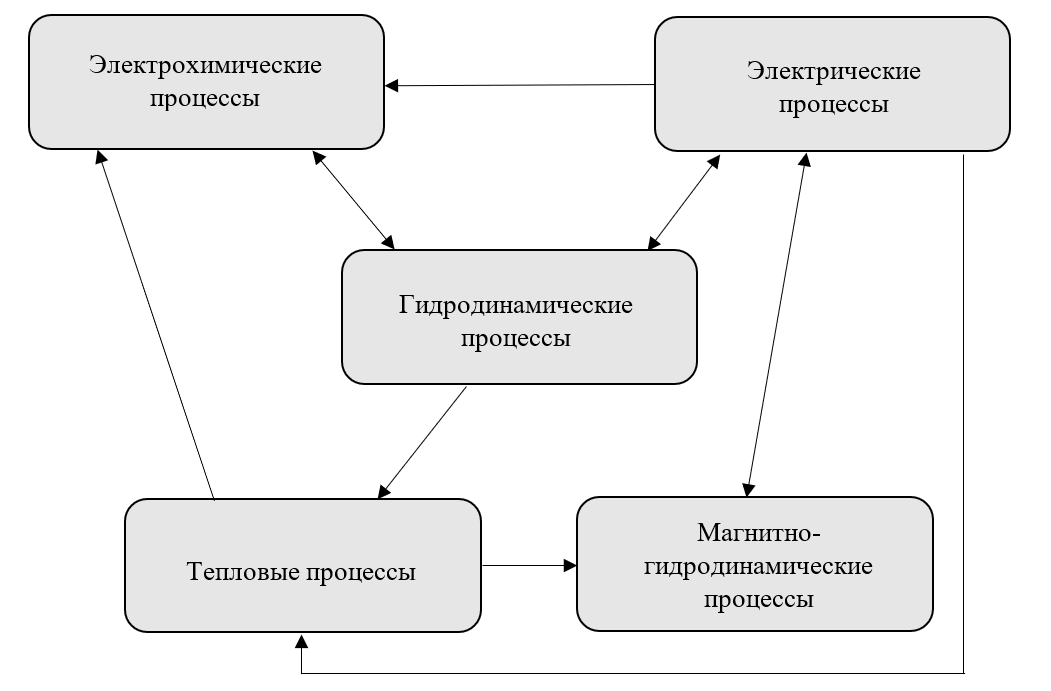
\includegraphics[width=1\linewidth]{схема взаимодействия.png}
    \caption{\label{fig:vliyanie} Взаимосвязь динамических процессов.}
\end{figure}

\begin{figure}[h]
    \centering
    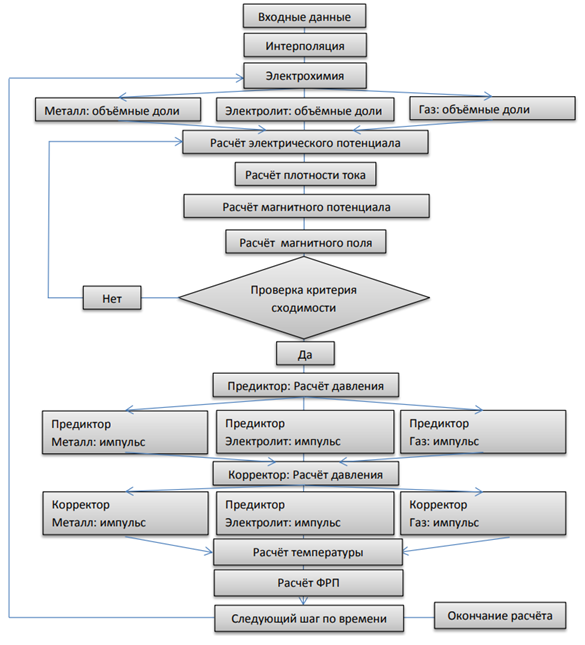
\includegraphics[width=1\linewidth]{блоксхема.png}
    \caption{\label{fig:vliyanie} Блок-схема вычислительного комплекса.}
\end{figure}

Для вычисления КО в любой интересующий момент времени требуется знать концентрации алюминия, натрия и фтора (блок «Электрохимия»), а также объёмные доли металла, электролита и газа, распределение плотности тока, потенциала и скорости в расплаве электролита, рассчитывающиеся каждый в своём блоке (см. рис. 2.). 

Для определения значений концентраций ионов используется уравнение Нернста-Планка, которое описывает изменения концентрации анионов и катионов химических элементов, возникающих в результате процесса электролиза [2]. Однако это уравнение не учитывает скорости движения среды. В работе [3] приводится модифицированное уравнение Нернста-Планка, учитывающее скорость движения заряженных частиц:

\[\frac{\partial C_i}{\partial t} = D_i\nabla^{2}C_i+D_i\frac{z_iF}{RT}div\big(C_i \cdot grad\phi\big) - \overrightarrow{v} \cdot gradC_i,  
\eqno(1) \]
\\
В этом уравнении $\overrightarrow{v}$ – известная фиксированная скорость движения среды. 

При процессе электролиза алюминия распределение скорости движения среды является вихревым во всех плоскостях сечения рабочего пространства, интенсивно изменяется во времени и находится во взаимосвязи со всеми динамическими процессами в электролизной ванне, в том числе и с изменением распределения потенциала во времени. В настоящей работе авторы предлагают новую модификацию уравнения Нернста-Планка.

\section{Математическое моделирование криолитового отношения}

Ниже представлено модифицированное уравнение Нернста-Планка, которое используется для вычисления концентрации ионов, необходимых для расчёта КО

\[\frac{\partial C_i}{\partial t} = D_idiv\bigg(gradC_i + \frac{z_iF}{RT}C_igrad\phi\bigg) - div(C_i \overrightarrow{v}_{\text{эл}}),  \eqno(2) \]
\\
где $C_i$ – концентрация $i$-ого иона/катиона, $t$-время, $D_i$ – коэффициент диффузии $i$-ого иона/катиона, $z_i$ – заряд $i$-ого иона/катиона, $F$ – постоянная Фарадея, $R$ – универсальная газовая постоянная, $T$ – температура, $\phi$ – потенциал электростатического поля, $\overrightarrow{v}_\text{эл}$ – скорость ионов.

Граничные условия на аноде и катоде

\[ \big(\nabla C_i + K_i C_i \nabla \phi \big) \cdot \overrightarrow{n} = G_i, \eqno(3) \] 
\\
где $K_i$ – коэффициент, определяющийся типом ионов,  $G_i$ зависит от плотности анодного (катодного) тока, $\overrightarrow{n}$ – нормаль к границе.

Граничные условия на стенках ванны

\[ \big(\nabla C_i + K_i C_i \nabla \phi \big) \cdot \overrightarrow{n} = 0, \eqno(4) \]

Концентрация ионов натрия находится из условия электронейтральности среды

\[ \sum\limits_{i=1}^6 z_iC_i = 0. \]

Концентрацию ионов алюминия предлагается находить из уравнения 

\[ \frac{\partial C_{Al}}{\partial t} = \frac{j_a}{F} - div(C_{Al} \overrightarrow{v}_{\text{эл}}) \]
\\
где $j_a$ - плотность тока на аноде.

Начальные условия для каждого иона известны, начальные условия для алюминия определяются в зависимости от его фазовой доли. 

Таким образом математическая постановка задачи вычисления КО заключается в решении системы уравнений (2) с граничными условиями (3), (4). Потенциал $\phi(t,x,y,z)$ и скорость $v(t,x,y,z)$ находятся при помощи основного вычислительного комплекса в каждый момент времени.

Задача (2)-(4) решается разностным методом с помощью разностной схемы, при этом уравнение (2) аппроксимируется со вторым порядком точности по пространству и по времени.

Анализ проведённой серии численных экспериментов позволил изучить пространственное распределение КО. 
Ниже представлены результаты расчёта трёхмерной задачи в плоскостном срезе рабочего плоскости XY на глубине 3 см от подошвы анода. На рисунке 3 представлен график векторного поля скоростей в расплаве криолита на высоте 39 см от дна ванны (на расстоянии 3 см от подошвы анода). Можно заметить, что завихрения образуются по всей площади ванны: обводящий по периметру вихрь, а также интенсивные вихри в центре сечения.

На рисунке 4 представлено распределение значений КО. Все вычисленные значения КО соответствуют известному диапазону стабильной работы ванны (2.6-2.8) и подтверждается экспериментальными наблюдениями. 

\begin{figure}[h!]
    \centering
    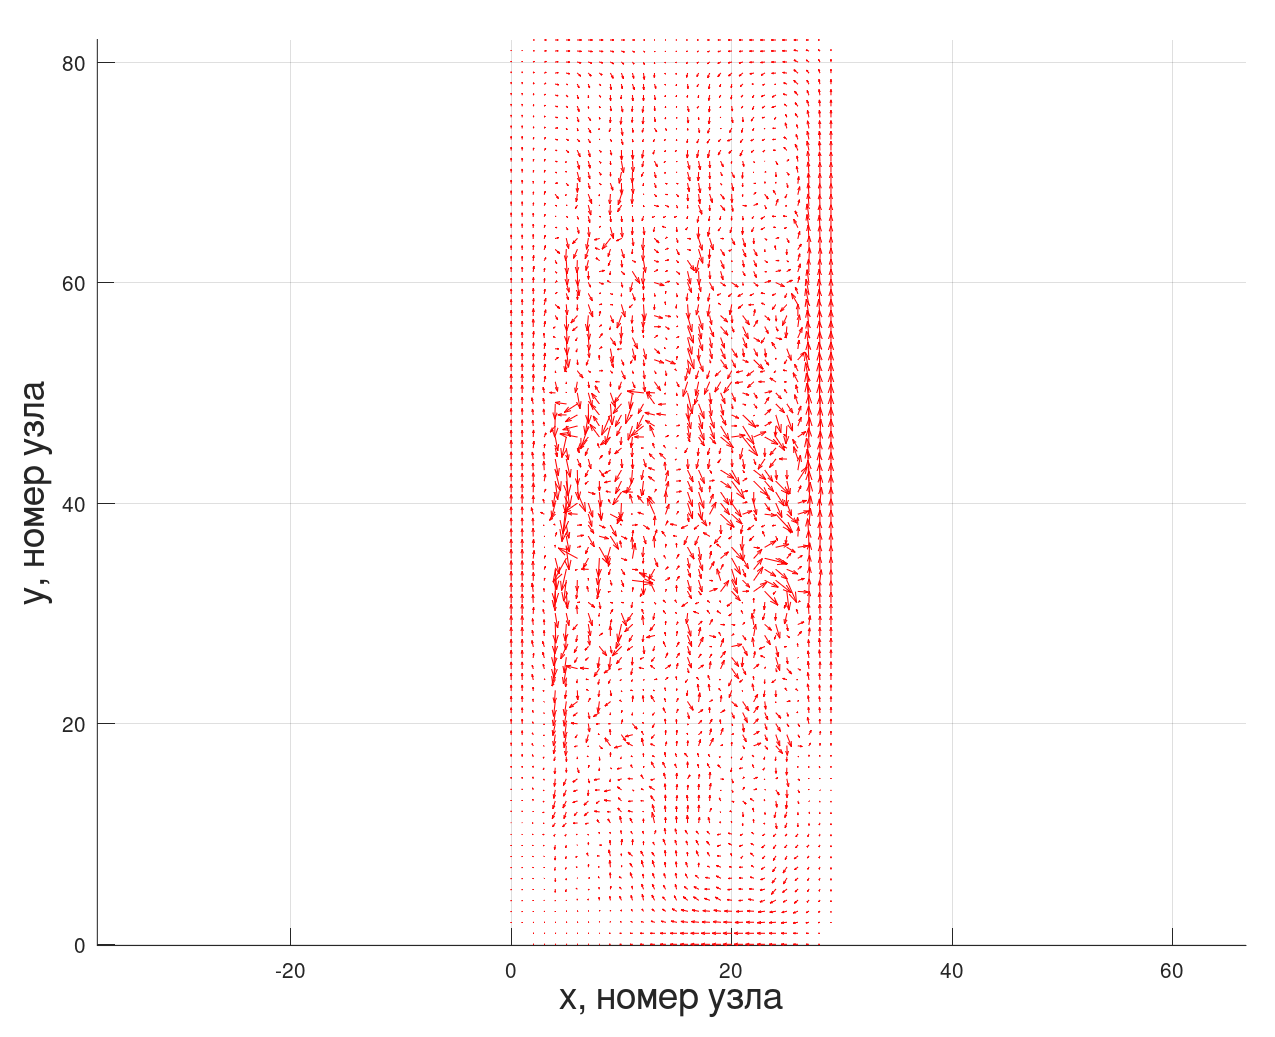
\includegraphics[width=110mm]{veloxy_art.png}
    \caption{Векторное поле скоростей в плоскости XY.}
    \label{fig:3dxyvelo} 
\end{figure}

\begin{figure}[h!]
    \centering
    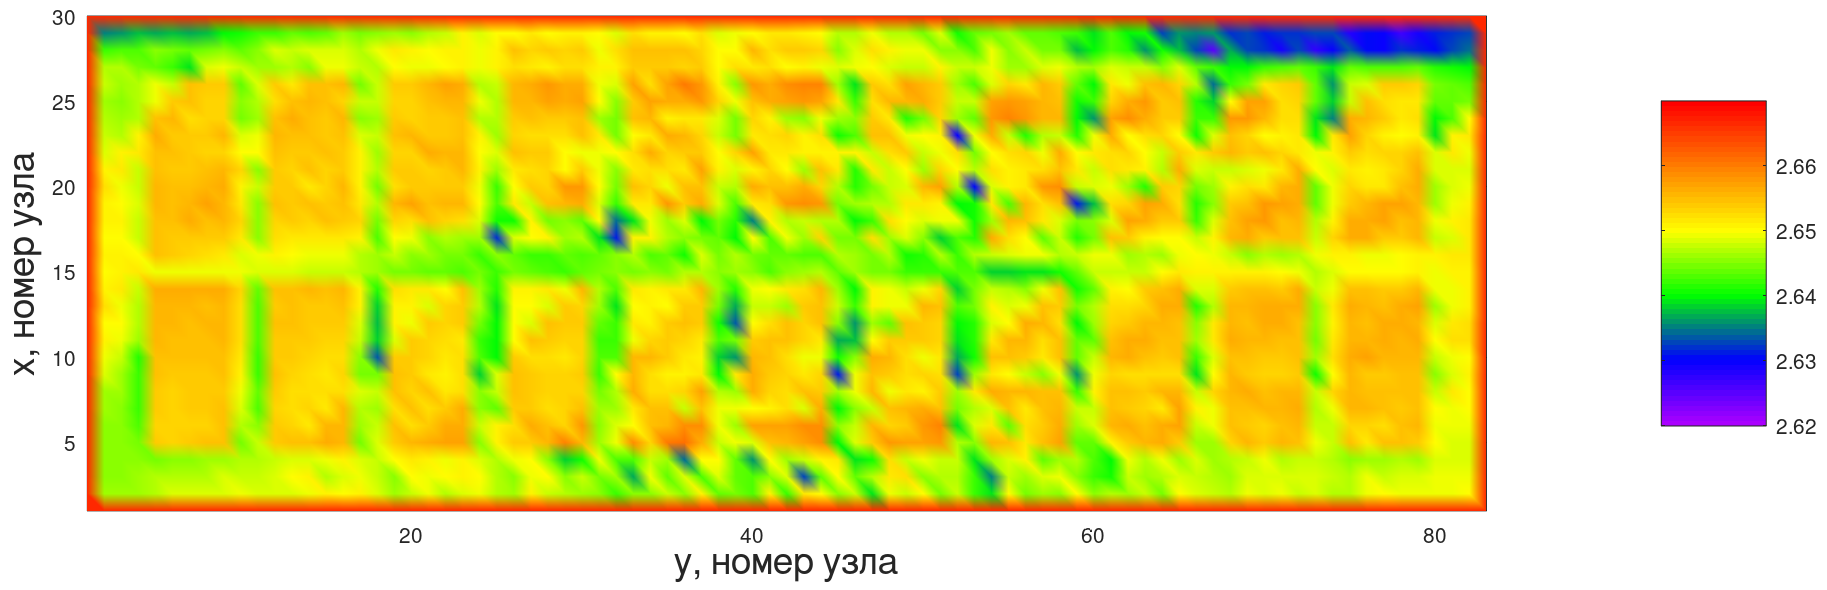
\includegraphics[width=90mm]{3d xy cr.png}
    \caption{Распределение значений криолитового отношения в плоскости XY.}
    \label{fig:3dxycr} 
\end{figure}

На рисунке 5 представлен график векторного поля скоростей в расплаве криолита. Наблюдается обводящий по периметру поток и небольшие вихревые образования у левого борта ванны.

Результаты численного эксперимента для сечения рабочего пространства плоскостью XZ на расстоянии 1,34 м от короткого борта промышленной ванны представлены на рисунке 6. Наглядно видно, что соответствующее распределение КО для скоростей, представленных на рис. 5, фактически однородно по всей плоскости сечения и принадлежит диапазону устойчивости работы ванны. 

\begin{figure}[h!]
    \centering
    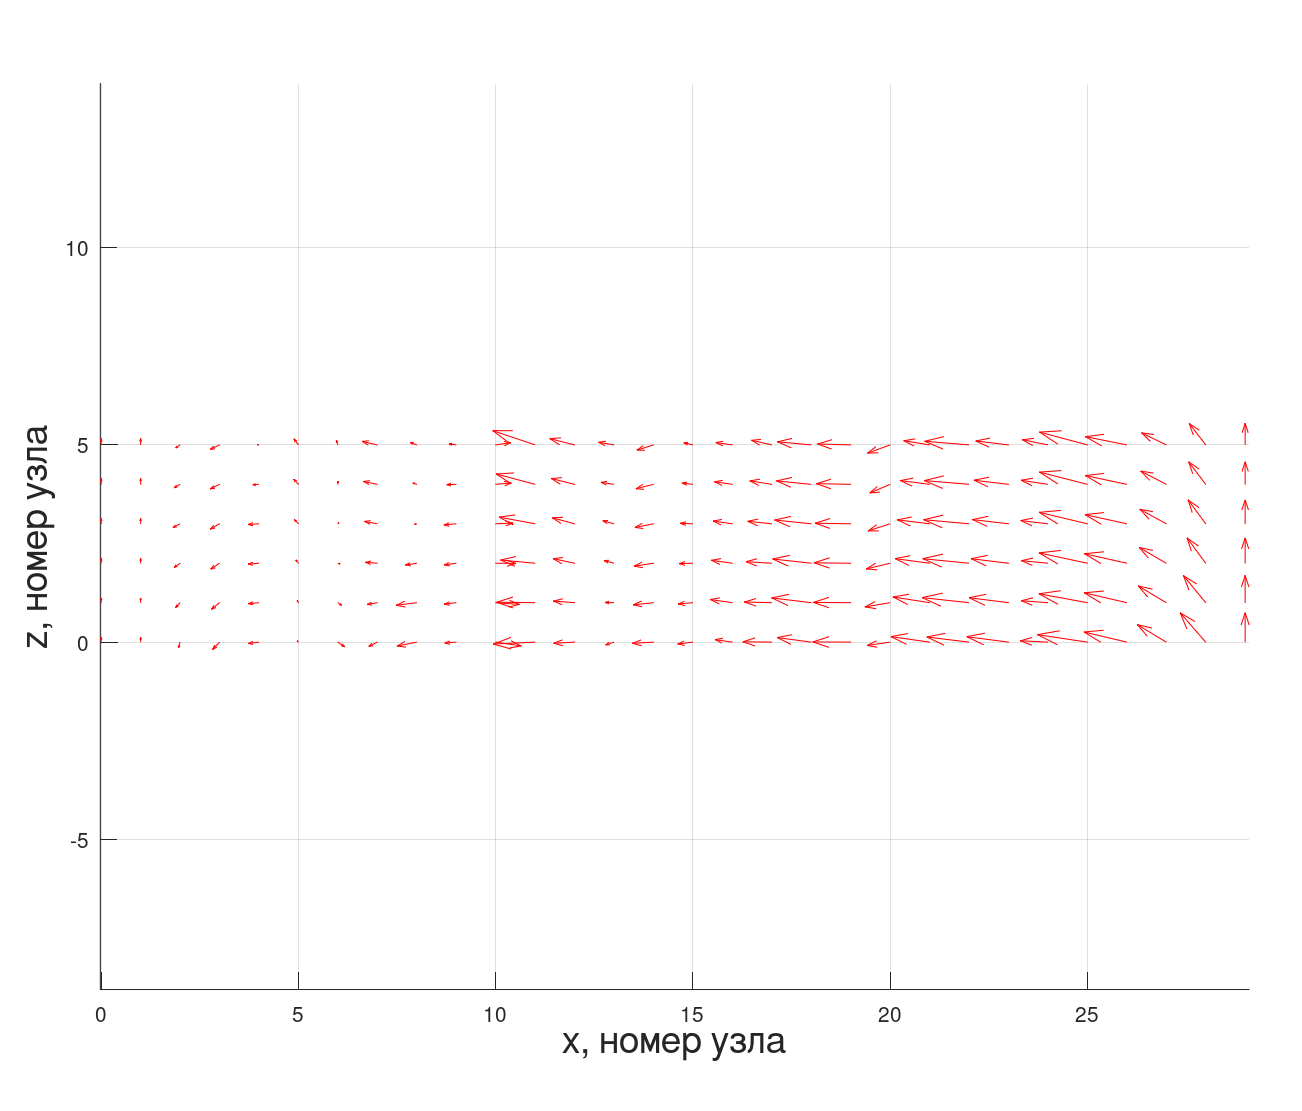
\includegraphics[width=110mm]{veloxz_art.png}
    \caption{Векторное поле скоростей в плоскости XZ.}
    \label{fig:3dxyvelo} 
\end{figure}

\begin{figure}[h!]
    \centering
    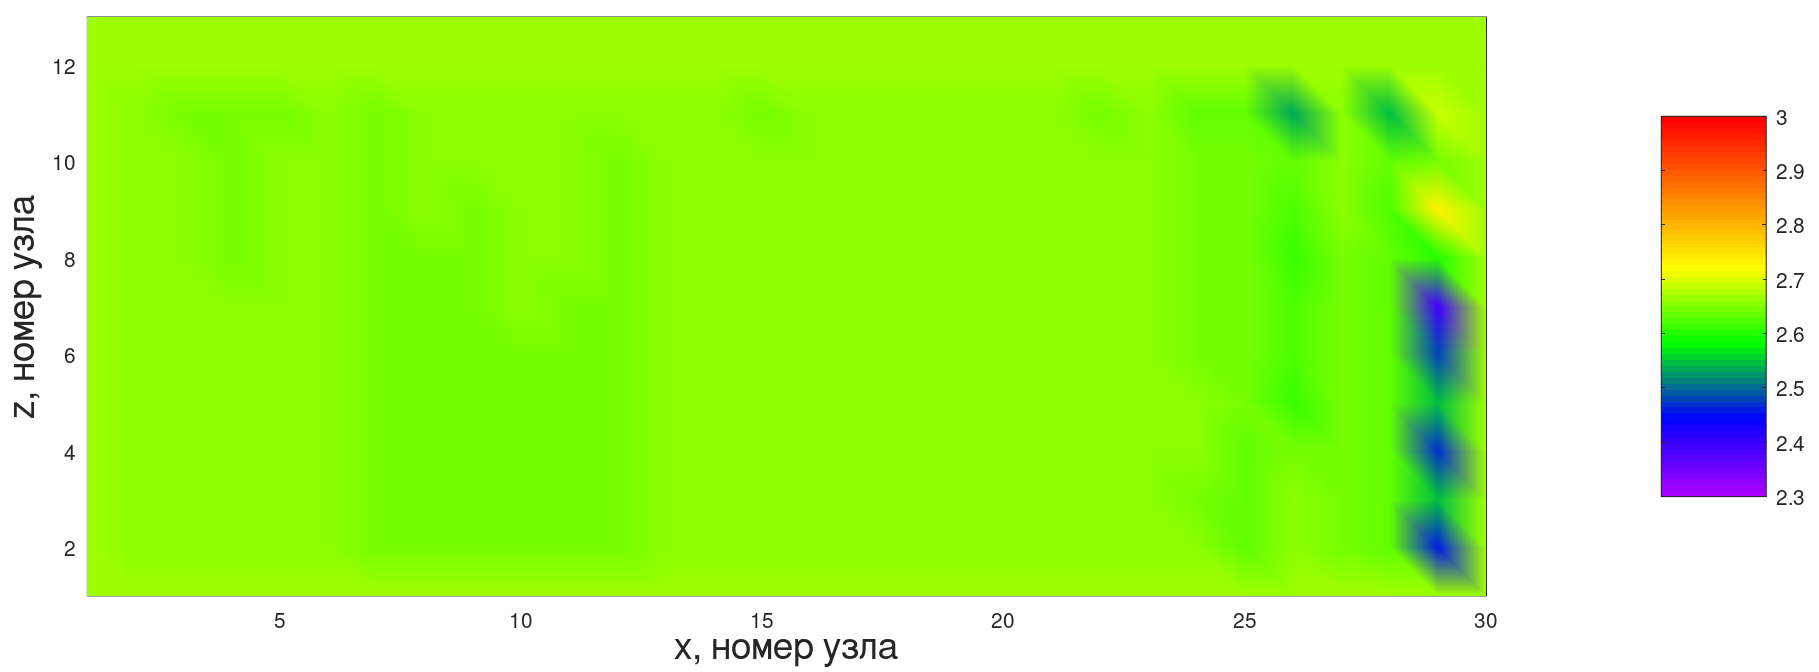
\includegraphics[width=90mm]{3d xz cr.png}
    \caption{Распределение значений криолитового отношения в плоскости XZ.}
    \label{fig:3dxycr} 
\end{figure}

На рисунках 7, 8 демонстрируются результаты численного эксперимента для сечения рабочего пространства плоскостью YZ, находящегося между длинным бортом и анодом на расстоянии 22 см от длинного борта промышленной ванны.	

На рисунке 7 представлен график векторного поля скоростей в расплаве криолита. Видно, что в этой плоскости значения скоростей невелики, вихрей не наблюдается. На рисунке 8 представлено соответствующее распределение значений КО.

Как и следовало ожидать, значения КО в плоскости сечения примерно одинаковы (КО = 2,65) и входят в диапазон значений устойчивой работы ванны. 

Таким образом, вихревые образования в поле распределения скоростей приводят к неоднородному распределению КО в рабочем пространстве. На практике это означает, что результат химического анализа взятой пробы сильно зависит от места взятия пробы в случае наличия вихревого движения скоростей и не зависит от места взятия пробы в случае безвихревого движения среды.

\begin{figure}[h!]
    \centering
    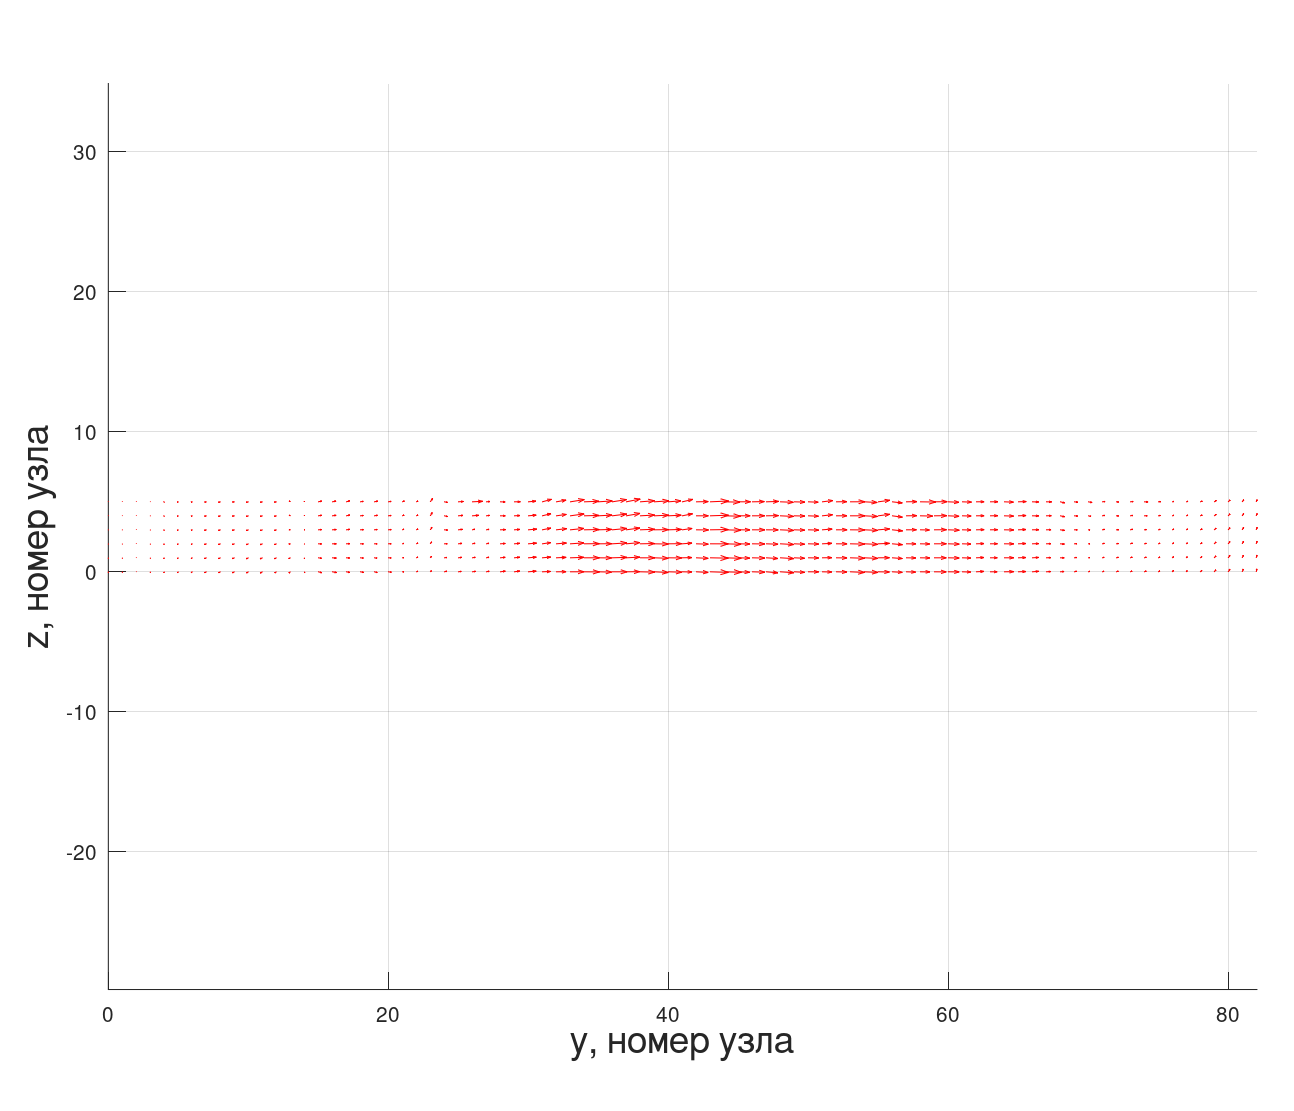
\includegraphics[width=110mm]{veloyz_art.png}
    \caption{Векторное поле скоростей в плоскости XZ.}
    \label{fig:3dxyvelo} 
\end{figure}

\begin{figure}[h!]
    \centering
    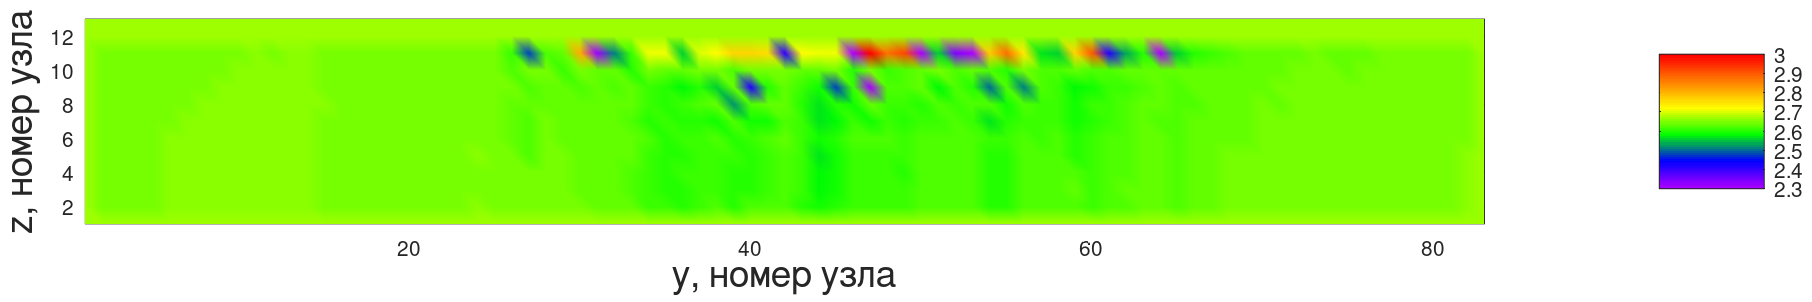
\includegraphics[width=90mm]{3d yz cr.png}
    \caption{Распределение значений криолитового отношения в плоскости XZ.}
    \label{fig:3dxycr} 
\end{figure}

\section{Вычисление управляющих параметров выхода по току и потери выхода по току}

Управляющие параметры выхода по току η и потери выхода по току $\Delta \eta$ наглядно отражают эффективность выхода по току алюминия при различных режимах работы электролизной ванны.

Теоретическое количество алюминия, которое должно получиться при электролизе, вычисляется по закону Фарадея

\[ M = F \cdot I \cdot t, \eqno(5) \]
\\
где $F$ - постоянная Фарадея, $I$ - сила тока, $t$ - время.

Однако количество произведённого металла всегда несколько меньше теоретического значения.

Экспериментальные исследования показывают, что выход по току η зависит от большого числа параметров: температуры, межполюсного расстояния (МПР) - расстояния между подошвой анода и границей раздела сред металл-электролит, плотности тока, геометрии рабочего пространства электролизёра, электромагнитных сил [4].

На практике в АСУТП применяется следующая эмпирическая формула [5] 

\[ \eta = \bigg(1-2567 \cdot \frac{S^{0,21}_{anod}}{i^{0,58}_{a}\cdot L_{ACD} \cdot e^{\frac{12940}{T_e}}}\bigg) \cdot 100, \]
\\
где 

При этом значения анодной плотности тока, температуры электролита и МПР определяются экспериментально в нескольких отдельных точках рабочего пространства ванны.
Таким образом точность вычисления выхода по току по формуле (6) напрямую зависит от точности входящих в неё параметров. Поскольку на практике значениям этих параметров соответствует большая погрешность, то величина η по формуле (6) вычисляется также с большой погрешностью. Трёхмерное трёхфазное математическое моделирование [6] позволяет исследовать распределение в рабочем пространстве ванны всех параметров, входящих в формулу (6), с достаточно большой точностью и изучить распределение $\eta$ и $\Delta\eta$, на основе которого можно сделать достаточно точную оценку эффективности производства алюминия в различные моменты времени.

В зависимости от режима работы электролизной ванны процесс электролиза может быть МГД-стабилен или МГД-нестабилен. В случае МГД-нестабильной работы ванны расстояние между анодом и катодом может быть критически мало, что ведёт к резкому уменьшению выхода по току. МГД-нестабильность всегда соответствует анодному эффекту (большое скопление углекислого газа под анодами, увеличивающего сопротивление среды), который происходит несколько раз в сутки. В случае многоанодной (22 анода) электролизной ванны МГД-нестабильность развивается в случае выемки и замены 11 и 22 анодов. В таблице 1 приводятся результаты вычисления величины выхода по току в моменты времени $t_1$ и $t_2$ $(t_2>t_1)$ при МГД-стабильности и МГД-нестабильности ванны. 

%тут должна быть таблица 1 (выход по току) (на самом деле 2 потому что свою я не сделал ещё)

\begin{figure}[h!]
    \centering
    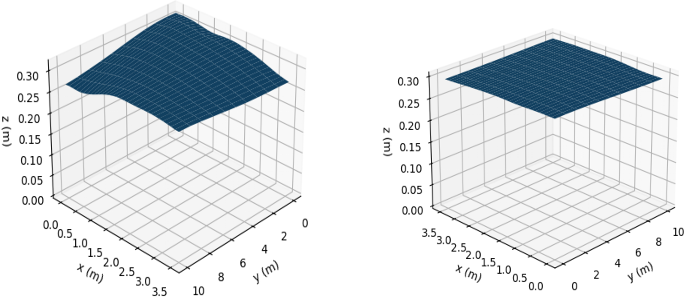
\includegraphics[width=90mm]{спокойная поверхность.png}
    \caption{Поверхность при МГД-стабильной работе ванны в моменты времени $t_1$(а) и $t_2$(б).}
    \label{fig:} 
\end{figure}

На рисунке 10 представлены поверхности раздела сред металл-электролит при выемке анодов в момент времени $t_1$ и $t_2$ для которых вычислялось значения выхода по току в таблице 1.

\begin{figure}[h!]
    \centering
    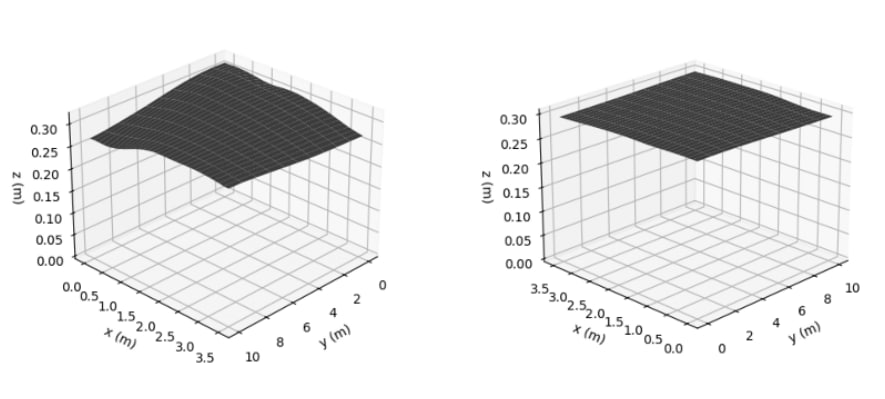
\includegraphics[width=90mm]{Выемка анодов поверхность.png}
    \caption{Поверхность при при выемке анодов.}
    \label{fig:} 
\end{figure}

На рисунке 11 представлены поверхности раздела сред металл-электролит при анодном эффекте в момент времени $t_1$ и $t_2$ для которых вычислялось значения выхода по току в таблице 1.

\begin{figure}[h!]
    \centering
    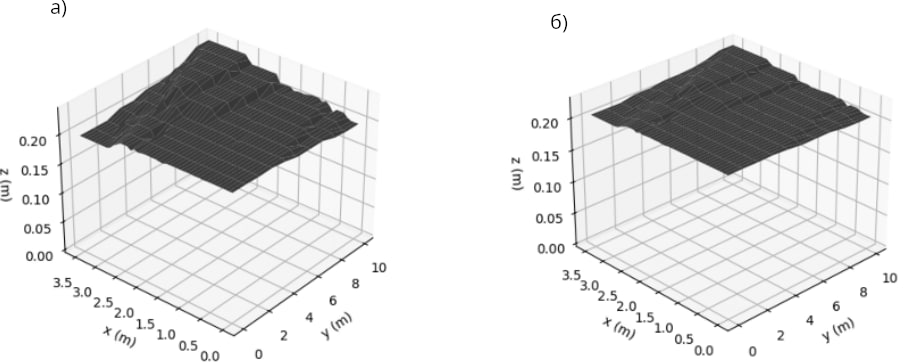
\includegraphics[width=90mm]{Анодный эффект поверхность.png}
    \caption{Поверхность при анодном эффекте.}
    \label{fig:} 
\end{figure}

Несмотря на то, что абсолютные значения изменения выхода по току и изменения потерь по току сильно отличаются, они имеют общую тенденцию на уменьшение выхода по току при искривлении поверхности. Такой результат можно было ожидать, поскольку формулы зависят от совершенно разных параметров, сильно связанных между собой в электролизёре в каждый момент времени, но по сути являющимися независимыми в расчётах по формуле (6). Например, при возникновении анодного эффекта резко возрастает за доли секунды напряжение, повышается температура в электролизёре, уменьшается плотность тока. При замене пары 11 и 22 анодов в электролизёре происходит перераспределение силы тока в ванне и рост амплитуды колебания границы раздела сред металл-электролит в области выемки анодов. В этих двух случаях за малое время невозможно провести замеры входящих в формулу (6) параметров. Тем не менее результаты, представленные в таблице 1, отражают общие тенденции по увеличению выхода по току при более стабильном режиме работы ванны.

В работе [8] представлена полуэмпирическая формула выхода по току

%

Однако практическая реализация формулы (7) зависит от точности определения поверхности раздела сред металл-электролит, а также требует достаточно точного вычисления поверхностного интеграла. 

При этом величина МПР, как и в формуле (6), определяется очень грубо (по характеру оплава опущенного в электролизную ванну стержня). Поэтому практическое использование формулы (7) весьма затруднительно. Более того, как показали проведённые в работе исследования, формула (7) является противоречивой, поскольку в случае выемки анодов (см. рис.10) в момент времени $t_2$, т.е. при спокойной поверхности раздела сред металл-электролит, значение  потерь выхода по току $\Delta\eta_2 = 0.0099$, а в момент времени $t_1$ при сильном возмущении границы раздела сред значение потери выхода по току $\Delta\eta_1 = 0.0074$, что противоречит здравому смыслу.  Таким образом, применение формулы (5) не является целесообразным.

Авторами предлагается модифицированная формула потерь выхода по току 

%
\\
в которой значения величин $l(x,y)$,$ H(x,y)$ в каждый момент времени определяются при помощи трёхмерного математического моделирования.

Вычисление поверхностного интеграла предлагается проводить при помощи метода триангуляции по формулам 

%

Точность вычисления поверхностного интеграла по формулам (9) – (12) имеет второй порядок и исследовалась численно на сгущающихся сетках.

Численный расчёт значений потерь выхода по току в случаях МГД-стабильной работы ванны $(\Delta\eta_1)$, при выемке анодов $(\Delta\eta_2)$ и анодном эффекте $(\Delta\eta_3)$ в момент времени $t_1$ показал, что 

\[ \Delta\eta_1 = 0.00674 < \Delta\eta_2 = 0.00945 < \Delta\eta_3 = 0.01188, \]
\\
откуда следует, что наибольшие потери выхода по току соответствуют анодному эффекту, а наименьшие – МГД-стабильному режиму работы ванны. Этот вывод соответствует практическим наблюдениям.

Аналогичные вычисления были проведены в момент времени $t_2$, которые показали, что
%исправить
\[ \Delta\eta_1 = 0.00674 < \Delta\eta_2 = 0.00945 < \Delta\eta_3 = 0.01188, \]

Процентные изменения потерь выхода по току в моменты времени t1 и t2 представлены в таблице 2. 

%таблица 2 изменение потерь по току

Из таблицы 2 видно, что наименьшие процентные потери соответствуют случаю МГД-стабильной работы ванны, когда поверхность раздела сред металл-электролит является наиболее спокойной (см. рис.9).
Ниже представлены результаты численных расчётов, иллюстрирующих распределение величины потери выхода по току в момент времени t1 и разных режимах работы ванны. Для каждого элементарного треугольника $\Delta^{1,2}_{i,j}$ проводится расчёт величины потери выхода по току $(\Delta\eta)_{i,j}$ для соответствующей формы поверхности раздела сред металл-электролит (см. рис. 9-11). На рис.12-14 представлены соответствующие распределения потерь выхода по току для границ раздела сред металл-электролит (рис.9-11) в случае МГД-стабильной и МГД-нестабильной работы ванны. 

\begin{figure}[h!]
    \centering
    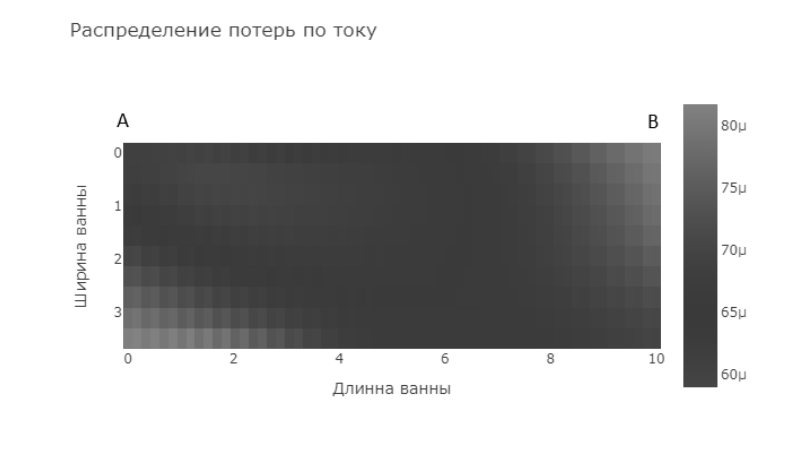
\includegraphics[width=90mm]{h.png}
    \caption{МГД-стабильный режим.}
    \label{fig:} 
\end{figure}

\begin{figure}[h!]
    \centering
    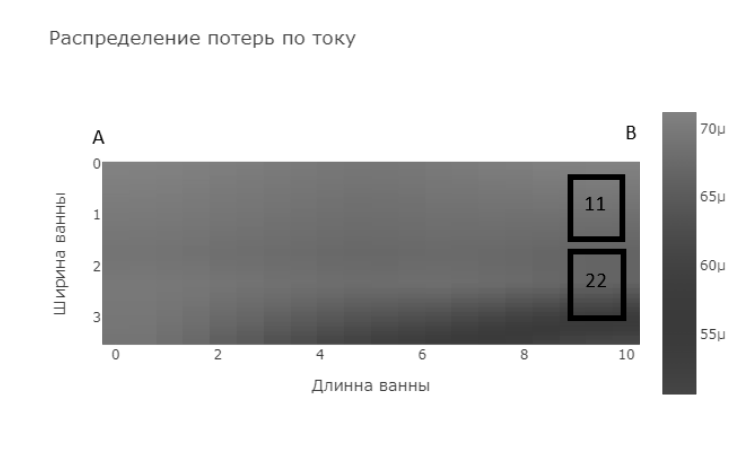
\includegraphics[width=90mm]{выемка анодов.png}
    \caption{Выемка анодов.}
    \label{fig:} 
\end{figure}

\begin{figure}[h!]
    \centering
    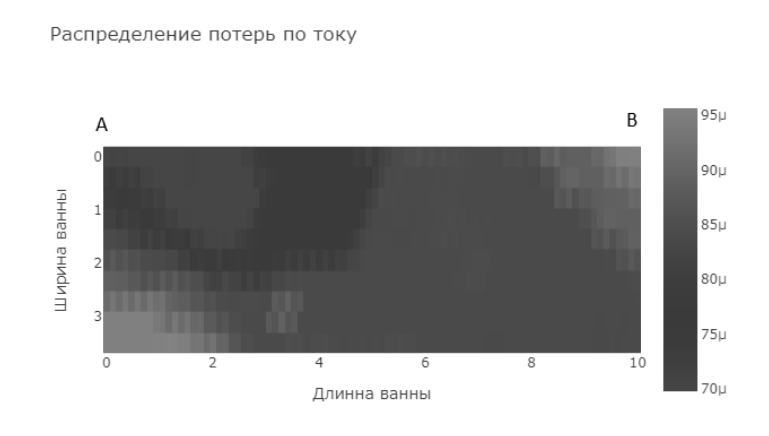
\includegraphics[width=90mm]{анодный эффект.png}
    \caption{Анодный эффект.}
    \label{fig:} 
\end{figure}

Анализ проведённых численных экспериментов позволяет сделать выводы о достоверности результатов лабораторных исследований стабильности режима работы ванны, которые проводятся при взятии отдельных проб.

\begin{thebibliography}{}
\end{thebibliography}

\end{document}